\documentclass[10pt]{article}

\usepackage[a4paper,margin=0.75in]{geometry}
\usepackage[T1]{fontenc}
\usepackage[utf8]{inputenc}
\usepackage{tgheros}
\usepackage{amssymb}
\renewcommand{\familydefault}{\sfdefault}
\usepackage{xcolor}
\definecolor{accent}{HTML}{3a9ade}
\definecolor{rule}{HTML}{BFC7CE}
\definecolor{muted}{HTML}{3a9ade}
\usepackage{titlesec}
\usepackage{enumitem}
\usepackage{graphicx}
\usepackage{wrapfig}
\usepackage[hidelinks,colorlinks=true,urlcolor=accent,linkcolor=accent]{hyperref}
\usepackage{fancyhdr}

\setlength{\parindent}{0pt}
\setlength{\parskip}{0pt}

\titleformat{\section}
  {\bfseries\large}
  {}{0em}{}
  [\vspace{1pt}{\color{rule}\titlerule[0.5pt]}]
\titlespacing*{\section}{0pt}{0.9em}{0.5em}

% date column + content column, used throughout
\newlength{\datecol}
\setlength{\datecol}{2.35cm}
\newcommand{\cvrow}[2]{%
  \noindent\begin{minipage}[t]{\datecol}\color{accent}\bfseries\small #1\end{minipage}%
  \begin{minipage}[t]{\dimexpr\linewidth-\datecol\relax}#2\end{minipage}\par\vspace{7pt}%
}
% bold 2-digit teal number + content, used for research work and publications
\newlength{\numcol}
\setlength{\numcol}{1.5em}
\newcommand{\cvnum}[2]{%
  \noindent\begin{minipage}[t]{\numcol}\color{accent}\bfseries #1\end{minipage}%
  \begin{minipage}[t]{\dimexpr\linewidth-\numcol\relax}#2\end{minipage}\par\vspace{7pt}%
}

% research plan: sub-heading style and hanging-indent list
\newcommand{\plansub}[1]{\par\vspace{0.9em}\noindent{\fontsize{11}{13.5}\selectfont\bfseries #1}\par\vspace{0.3em}}
\newenvironment{planlist}{\begin{list}{}{\setlength{\leftmargin}{2.2em}\setlength{\itemindent}{-2.2em}\setlength{\itemsep}{3pt}\setlength{\topsep}{3pt}\setlength{\parsep}{0pt}}}{\end{list}}

\pagestyle{empty}

\begin{document}

%---------------------------------------------------------
% Header
%---------------------------------------------------------
{\Huge\bfseries Zehong Liao}\\[0.3em]

\vspace{0.1em}
\section*{Personal Information}
\begin{itemize}[leftmargin=1.2em,itemsep=4pt,topsep=2pt,label={\color{accent}$\blacktriangleright$}]

\item \textbf{Name:} Zehong Liao

\item \textbf{Date:} July 15, 1998

\item \textbf{Nationality}: China

\item \textbf{Email} \href{mailto:liaozh26@mail2.sysu.edu.cn}{liaozh26@mail2.sysu.edu.cn}
\quad\textbf{Website} \href{https://murry-liao.github.io}{murry-liao.github.io}
\quad\textbf{GitHub} \href{https://github.com/murry-liao}{murry-liao}
\end{itemize}



%---------------------------------------------------------
\section*{Education \& Research Experience}

\cvrow{Sep 2021 -- \\ Jul 2026}{%
  \textbf{Sun Yat-sen University}, China \textperiodcentered\ PhD \textperiodcentered\ (Supervisor: Prof. Long Zhu)\\
  Sino-French Institute of Nuclear Engineering and Technology; 
}
\cvrow{Apr 2025 -- \\ Dec 2025}{%
  \textbf{Kyoto University}, Japan \textperiodcentered\ Research Visitor
  \textperiodcentered\ (Host: Prof. Kouichi Hagino)\\
  Department of Physics, Graduate School of Science;  
  %
}
\cvrow{Sep 2017 -- \\ Jun 2021}{%
  \textbf{North China Electric Power University}, China \textperiodcentered\ B.Sc.\\
  Nuclear Science and Technology.%
}

%---------------------------------------------------------
\section*{Graduate Awards}

\cvrow{2026.6}{\textbf{Outstanding Graduate of Sino-French Institute of Nuclear Engineering and Technology} }

\cvrow{2024.11}{\textbf{Student Outstanding Report Award} \textperiodcentered\ 3rd Symposium on Nuclear Physics in the Guangdong--Hong Kong--Macao Greater Bay Area, Shenzhen, China}




%---------------------------------------------------------
\section*{Academic meeting  \&  Talks(Selected)}

\cvrow{2026.10}{\textbf{A unified description of low-energy fusion and multinucleon-transfer
  reactions within the Coupled Master--Langevin model} \textperiodcentered\ Seminar, Department of
  Physics, Kyoto University}
\cvrow{2025.12}{\textbf{Determination of nuclear deformations with an emulator for sub-barrier
  fusion reactions} \textperiodcentered\ 10th Kansai Nuclear Many-Body Seminar, Osaka Metropolitan
  University, Japan}
\cvrow{2024.11}{\textbf{Angular distribution in the multinucleon transfer reaction}
  \textperiodcentered\ 3rd Symposium on Nuclear Physics in the Guangdong--Hong Kong--Macao Greater
  Bay Area, Shenzhen, China}
\cvrow{2024.10}{\textbf{Angular distribution in the multinucleon transfer reaction}
  \textperiodcentered\ 2nd Multinucleon Transfer Reactions Symposium, Changsha, China}
%---------------------------------------------------------

\section*{Open Source \& Research Software}
\textbf{Coupled-channels model \& emulator:} Fortran 90 / Python solver for heavy-ion fusion
coupled-channels calculations and reduced-basis emulator development; includes a rewrite of
CCFULL and multiple numerical solution methods.
\href{https://github.com/murry-liao/CCFULL_ReduceBasisMethod_Emulator}{Project repository}\\[3pt]
\textbf{Nuclear potential surface:} Fortran program for Coulomb-barrier and
potential-energy-surface description
\href{https://murry-liao.github.io/file_code/}{Project repository}
%---------------------------------------------------------

%\newpage
\pagestyle{fancy}
\fancyhf{}
\renewcommand{\headrulewidth}{0pt}
\fancyhead[R]{\footnotesize\color{muted} ZEHONG LIAO \ /\ ACADEMIC CV \ /\ 2026}
\fancyfoot[C]{\footnotesize\color{muted} Zehong Liao \textbar\ ACADEMIC CV \ \textperiodcentered\ \ \thepage}

%---------------------------------------------------------
\newpage
\section*{List of publications}
\textit{13 publications in total; 6 first-author papers and 7 collaborative works
are listed below.}
\vspace{5pt}

\cvnum{01}{\textbf{Determination of nuclear deformations with an emulator for sub-barrier fusion
  reactions} \\
  \underline{Z.~H.~Liao}, K. Hagino, L. Zhu, S. Yoshida, K. Uzawa.
  Phys. Rev. C \textbf{113}, 044611 (2026).
  \textperiodcentered\ \href{https://journals.aps.org/prc/abstract/10.1103/8ycb-lrqq}{DOI}}

\cvnum{02}{\textbf{Mechanism of the quasielastic scattering based on the dinuclear system concept}
  \textcolor{accent}{[Letter]}\\
  \underline{Z.~H.~Liao}, Y. Yang, Z. P. Gao, J. Su, L. Zhu.
  Phys. Rev. C \textbf{112}, L051601 (2025).
  \textperiodcentered\ \href{https://doi.org/10.1103/yfkd-w7gs}{DOI}}

\cvnum{03}{\textbf{Quantifying angular distributions in multinucleon transfer reactions with a
  semiclassical method} \\
   \underline{Z.~H.~Liao}, Z. P. Gao, Y. Yang, Y. P. Fang, L. Zhu, J. Su.
  Phys. Rev. C \textbf{111}, 024605 (2025).
  \textperiodcentered\ \href{https://journals.aps.org/prc/abstract/10.1103/PhysRevC.111.024605}{DOI}}

\cvnum{04}{\textbf{Shell effects on the drift and fluctuation in multinucleon transfer reactions}
  \\
  \underline{Z.~H.~Liao}, Z. P. Gao, Y. Yang, L. Zhu, J. Su.
  Phys. Rev. C \textbf{109}, 054612 (2024).
  \textperiodcentered\ \href{https://journals.aps.org/prc/abstract/10.1103/PhysRevC.109.054612}{DOI}}

\cvnum{05}{\textbf{Optimal detection angles for producing $N=126$ neutron-rich isotones in
  multinucleon transfer reactions} \textcolor{accent}{[Letter]}\\
  \underline{Z.~H.~Liao}, L. Zhu, Z. P. Gao, J. Su, C. Li.
  Phys. Rev. Research \textbf{5}, L022021 (2023).
  \textperiodcentered\ \href{https://journals.aps.org/prresearch/abstract/10.1103/PhysRevResearch.5.L022021}{DOI}}

\cvnum{06}{\textbf{Dynamics of charge equilibration and effects on producing neutron-rich isotopes
  around $N=126$ in multinucleon transfer reactions} \\
  \underline{Z.~H.~Liao}, L. Zhu, J. Su, C. Li.
  Phys. Rev. C \textbf{107}, 014614 (2023).
  \textperiodcentered\ \href{https://journals.aps.org/prc/abstract/10.1103/PhysRevC.107.014614}{DOI}}

\cvnum{07}{\textbf{Correlation of multiple physical quantities in multinucleon transfer reactions:
  insight into production of isotopes near the shell closure $N=152$}
  \textcolor{accent}{[Co-author \textperiodcentered\ Editors' Suggestion]}\\
   Z. M. Shen, \underline{Z.~H.~Liao}, L. Zhu.
  Phys. Rev. C \textbf{113}, L021601 (2026).
  \textperiodcentered\ \href{https://doi.org/10.1103/xbtz-bvmc}{DOI}}

\cvnum{08}{\textbf{Emulating multichannel scattering based on eigenvector continuation in the
  discrete-basis formalism} \\
  K. Hagino, \underline{Z.~H.~Liao}, S. Yoshida, M. Kimura, K. Uzawa.
  Phys. Rev. C \textbf{112}, 024618 (2025).
  \textperiodcentered\ \href{https://journals.aps.org/prc/abstract/10.1103/zpsz-7jld}{DOI}}

\cvnum{09}{\textbf{Production of actinide isotopes near $\theta_{\mathrm{lab}}=0^{\circ}$ in
  multinucleon transfer
  reaction \textsuperscript{238}U + \textsuperscript{248}Cm} \\
  Y. Yang, L. Zhu, \underline{Z.~H.~Liao}, Z. P. Gao, Y. P. Fang, J. Su, Z. Liu, D. S. Hou, H. Huang, C. Li,
  F. S. Zhang.\\ \mbox{Phys. Lett. B \textbf{862}, 139318 (2025).
  \textperiodcentered\ \href{https://doi.org/10.1016/j.physletb.2025.139318}{DOI}}}

\cvnum{10}{\textbf{New insight into the N/Z and mass equilibration in heavy-ion collisions}
  \\
  Y. Yang, \underline{Z.~H.~Liao}, Z. P. Gao, L. Zhu, J. Su, C. Li.
  Phys. Rev. C \textbf{111}, 024602 (2025).
  \textperiodcentered\ \href{https://journals.aps.org/prc/abstract/10.1103/PhysRevC.111.024602}{DOI}}

\cvnum{11}{\textbf{Bayesian uncertainty quantification for synthesizing superheavy elements}
 \\
  Y. P. Fang, Z. P. Gao, Y. N. Zhang, \underline{Z.~H.~Liao}, Y. Yang, J. Su, L. Zhu. \mbox{Phys. Lett. B
  \textbf{858}, 139069 (2024).
  \textperiodcentered\ \href{https://doi.org/10.1016/j.physletb.2024.139069}{DOI}}}

\cvnum{12}{\textbf{Role of the isospin diffusion on the cluster transfer in \textsuperscript{12,14}C + \textsuperscript{209}Bi
  reactions} \textcolor{accent}{\mbox{[Letter]}}\\
  Z. P. Gao, Y. N. Zhang, L. Zhu, \underline{Z.~H.~Liao}, Y. Yang, C. C. Guo, J. Su.\\ \mbox{Phys. Rev. C
  \textbf{109}, L041605 (2024).
  \textperiodcentered\ \href{https://journals.aps.org/prc/abstract/10.1103/PhysRevC.109.L041605}{DOI}}}

\cvnum{13}{\textbf{Constraining the Woods--Saxon potential in fusion reactions based on the
  neural network} \\
  Z. P. Gao, S. Y. Liu, P. W. Wen, \underline{Z.~H.~Liao}, Y. Yang, J. Su, Y. J. Wang, L. Zhu.\\ \mbox{Phys. Rev. C
  \textbf{109}, 024601 (2024).
  \textperiodcentered\ \href{https://journals.aps.org/prc/abstract/10.1103/PhysRevC.109.024601}{DOI}}}





%---------------------------------------------------------
\newpage
\section*{Research history}
I have finished my PhD degree at
\textbf{Sun Yat-sen University, China (July 2026).} My research focuses on low-energy nuclear physics, aiming to understand how nuclei are produced and how nuclear structure affects reaction dynamics. During my PhD, I published six articles in Physical Review C and Physical Review Research. My work can be broadly divided into three research directions:
\begin{itemize}[leftmargin=1.2em,itemsep=4pt,topsep=2pt,label={\color{accent}$\blacktriangleright$}]
\item \textbf{The study of multi-nucleon transfer (MNT) reactions to expand the nuclear chart.}

Exotic nuclei which do not exist naturally must be produced through nuclear reactions. For this purpose, multi-nucleon transfer (MNT) reactions are regarded as a promising approach to explore the unknown $N=126$ nuclei [1]. Here, MNT is defined as a reaction in which many nucleons (protons and neutrons) are transferred from one nucleus to the other nucleus during the reaction. In most cases, this is accompanied by a significant loss of kinetic energy and a wide angular distribution in the exit channel. While these challenges remain very significant, they have not been well understood for a practical application of MNT reactions to produce exotic nuclei.

In this area of research, I applied and further developed the dinuclear system model to investigate MNT reactions. In this model, the nuclear reaction potential energy surface is first constructed using the macroscopic–microscopic approach and then a master equation is solved to obtain the probability distribution of reaction products [2]. I successfully showed that the model effectively describes the cross sections of MNT reactions. Moreover, I quantitatively predicted production cross-sections and angular distributions of unknown nuclides, particularly in the neutron-rich $N=126$ region, and proposed optimal projectile-target combinations, incident energies, and detector angles [3, 4, 5]. These works are important, as they have provided theoretical guidance for experimental design, enabling efficient detection.

\item \textbf{Fusion reactions and the extraction of nuclear deformation.} 

It has been well recognized that many nuclei are deformed in the ground state. Such nuclear deformation plays an important role in low-energy heavy-ion fusion reactions. For instance, the static deformation of nuclei strongly affects experimental observables such as fusion cross sections. Using this property, nuclear deformation parameters can be extracted by comparing experimental data with theoretical calculations based on the coupled-channels model, which is a quantum mechanical reaction theory for multi-channel problems [6]. However, traditional coupled-channels calculations require extensive computations when many parameters are involved. To address this problem, I successfully constructed a Coupled-Channels emulator based on the Reduced Basis method (Eigenvector Continuation). This approach significantly accelerates the calculation while maintaining high accuracy [7]. Applying this method to heavy-ion fusion reactions for systems such as \textsuperscript{16}O +  \textsuperscript{144,154}Sm and \textsuperscript{16}O + \textsuperscript{186}W, I successfully extracted the nuclear deformation parameters of the target nuclei. This work has provided an efficient theoretical tool for systematically exploring intrinsic nuclear shapes through nuclear reactions [8, 9]. This work was carried out with my host Prof. Kouichi Hagino during my stay at Kyoto University in 2025.

\item \textbf{Nuclear Reaction Computation Methods} 

Stable and efficient numerical methods are crucial for solving the coupled-channels equations. I developed several numerical methods for solving the coupled-channels equations, including the modified Numerov method, the R-matrix method, and the discrete-basis method. I also have developed a reduced-basis emulator for the coupled-channels model, which can significantly accelerate the calculation of fusion cross sections. 

\textbf{Reference:}

[1]. Y. X. Watanabe, Y. H. Kim, S. C. Jeong, et al., Physical Review Letters 115, 172503 (2015)

[2]. L. Zhu, J. Su, W. J. Xie and F. S. Zhang, Physics Letters B 767 (2017) 437–442

[3]. Z. H. Liao, L. Zhu, J. Su and C. Li, Physical Review C 107, 014614 (2023)

[4]. Z. H. Liao, L. Zhu, Z. P. Gao, J. Su and C. Li, Physical Review Research 5, L022021 (2023)

[5]. Z. H. Liao, Z. P. Gao, Y. Yang, L. Zhu and J. Su, Physical Review C 109, 054612 (2024)

[6]. Y. K. Gupta, V. B. Katariya, G. K. Prajapati, K. Hagino, et al., Physics Letters B 845 (2023) 138120

[7]. D. Frame, R. Z. He, I. Ipsen, D. Lee, D. Lee and E. Rrapaj, Physical Review Letters 121, 032501 (2018)

[8]. K. Hagino, Z. H. Liao, S. Yoshida, M. Kimura, K. Uzawa, et al., Physical Review C 112, 024618 (2025) 

[9]. Z. H. Liao, K. Hagino, L. Zhu, S. Yoshida, K. Uzawa, et al., Physical Review C 113, 044611 (2026)

\end{itemize}



%---------------------------------------------------------
\newpage
\section*{Research plan}
\setlength{\parskip}{4pt}

\plansub{Background of proposed research plan}

\begin{wrapfigure}{r}{0.5\linewidth}
  \centering
  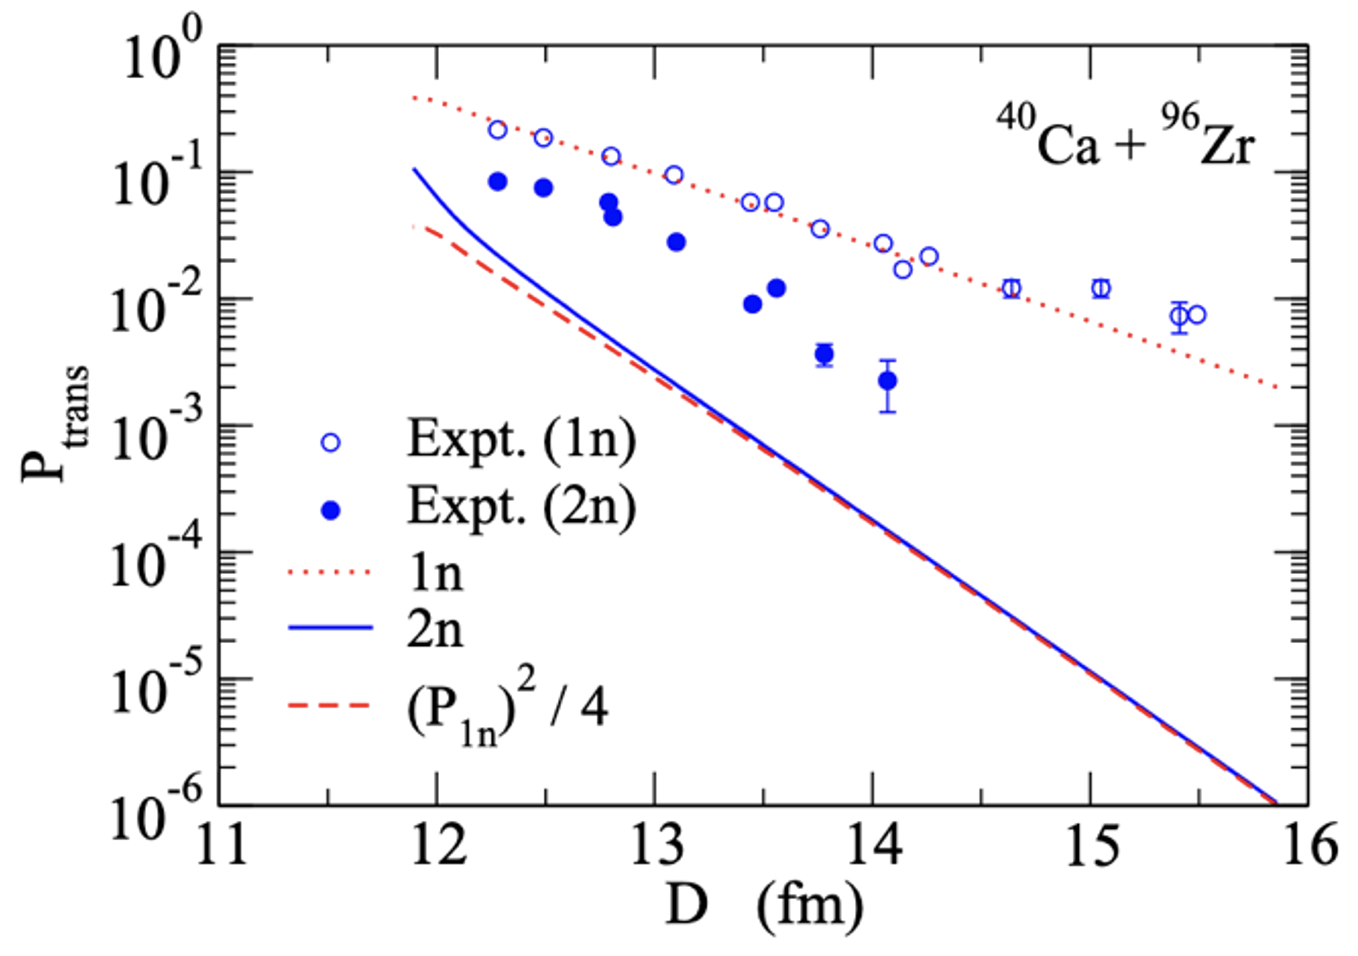
\includegraphics[width=\linewidth]{Fig1.png}
  \caption{The Experimental (points) and calculated (lines) transfer probabilities for the one- and two-nucleon pickup. This figure comes from [2]}
\end{wrapfigure}

Pairing correlation has been considered a fundamental correlation in nuclear many-body systems. It has been regarded to be closely related to two-particle transfer reactions. Crucially, many experimental data reveal a macroscopic enhancement [1] in two-particle transfer cross sections compared to estimates derived from the independent-particle transfer picture—specifically, the two-neutron transfer probability significantly exceeds the square of the single-neutron transfer probability, as shown in Fig. 1 [2]. Thus, two-particle transfer reactions far below the Coulomb barrier serve as powerful probes for investigating
nucleon-nucleon correlations and the possible manifestation of a nuclear Josephson effect, i.e., the tunneling of Cooper pairs between superfluid nuclei [3]. However, a comprehensive theoretical description of these reactions remains a major challenge. Although several reaction models have been developed, such as the distorted-wave Born approximation and coupled-channels approaches, these methods usually rely on simplifying assumptions and phenomenological inputs. In particular, important effects such as pairing correlations and the non-orthogonality between transfer channels are often treated approximately. As a result, existing models are not yet able to provide a fully microscopic and quantitative description of experimental data.

\plansub{Purpose of proposed research}

Therefore, a fully microscopic and quantitative description of pair transfer reactions remains an open problem. The goal of this project is to develop a unified theoretical framework combining the time-dependent solution of the Schrödinger equation (TDSE) [4] and time-independent coupled-channels (CC) theory [5] to investigate two-particle transfer reactions. The overall research framework is illustrated in Fig. 2.
In this project, the exact solutions obtained from the TDSE for simplified
models will provide a more realistic description of the reaction dynamics
and spatial correlations. And we can use it as a reference to test different
approximation schemes involved in the CC formalism. At the same time,
the time-independent coupled-channels framework will be improved by incorporating microscopic overlap functions for transfer couplings [6]. Non-orthogonality effects in the transfer channels will be also explicitly included, allowing for a more consistent description of two-particle transfer mechanisms.
To quantitatively validate pair transfer induced by pair correlations, these methods will be applied to the \textsuperscript{96}Zr + \textsuperscript{40}Ca, \textsuperscript{116}Sn + \textsuperscript{60}Ni, and \textsuperscript{206}Pb + \textsuperscript{118}Sn systems. Systematic comparisons between our theoretical calculations and these existing experimental data will provide a solid ground to evaluate the microscopic description of nn, pp, and pn pairing correlations.

\plansub{Proposed plan}

\textbf{First year:} In the first half of the year, the applicant will begin implementing the time-dependent solution of the Schrödinger equation for a simplified model describing two-particle transfer reactions, inspired by Ref. [4]. This model will allow an exact solution of the reaction dynamics, which will be used as a benchmark. In the second half of the year, the applicant will investigate how pairing correlations and spatial correlations of a cooper pair influence the transfer probabilities. These results will provide guidance for constructing realistic transfer couplings in the coupled-channels approach.
\par\textbf{Second year:} The time-independent coupled-channels framework will be improved by incorporating pair transfer coupling via microscopic overlap function. In particular, the effects of pairing correlations and non-orthogonality in the transfer channels will be explicitly included. The developed framework will then be applied to the analysis of two-particle transfer reactions such as \textsuperscript{96}Zr + \textsuperscript{40}Ca, \textsuperscript{116}Sn + \textsuperscript{60}Ni, and \textsuperscript{206}Pb + \textsuperscript{118}Sn. Systematic calculations of transfer probabilities and cross sections will be performed and compared with available experimental data. At the same time, the applicant will analyze the nn, pp, and pn pairing correlations within the same model. This will offer reliable theoretical understanding for the pair transfer reaction.

\plansub{Expected results and impacts}

The proposed research is expected to establish a unified theoretical framework for the microscopic description of two-particle transfer reactions at sub-barrier energies by combining the time-dependent solution of the Schrödinger equation with time-independent coupled-channels theory.
\par\begin{planlist}
\item[] (1) By incorporating pairing correlations and non-orthogonality effects in a microscopic manner, the developed model will provide a more realistic description of neutron-neutron, proton-proton, and proton-neutron pair transfer processes. The results are expected to clarify the dynamical role of nucleon pairing correlations in heavy-ion reactions and improve the quantitative interpretation of experimental transfer data.
\item[] (2) The proposed framework will be applied to reactions such as \textsuperscript{96}Zr + \textsuperscript{40}Ca, \textsuperscript{116}Sn + \textsuperscript{60}Ni, and \textsuperscript{206}Pb + \textsuperscript{118}Sn, where experimental data are available. Systematic comparisons between theoretical predictions and experimental observations will provide new insights into the mechanisms of pair transfer at sub-barrier energies.
\item[] (3) The new method will provide a useful wool to investigate the pairing correlation in neutron-rich nuclei, for which the pairing correlation plays a crucial role in its description.
\item[] (4) More broadly, this research will contribute to a deeper understanding of nuclear pairing correlations and their role in nuclear reactions. The relevant code will be released and published, providing a reliable tool for analyzing future experiments.

\end{planlist}
\setlength{\parskip}{0pt}
\plansub{Reference:}

[1]. L. Corradi, EPJ Web of Conferences 306, 01015 (2024)

[2]. K. Hagino and G. Scamps, Physical Review C 92, 064602 (2015)

[3]. D. Montanari, L. Corradi et al., Physical Review Letters 113, 052501 (2014)

[4]. L. Moschini et al., Physical Review C 103, 014604 (2021)

[5]. G. Scamps and K. Hagino, Physical Review C 92, 054614 (2015)

[6]. J. M. Bang et al., Physics Reports 125(6), 253--399 (1985)


\end{document}
